% Pacotes e configurações padrão do estilo ``article''\
% -------------------------------------
\documentclass[a4paper,11pt]{article}
% Layout
% ------------------------------------------------------------------------------
%     Gráficos e layout ----------------------------------------------------------------------

\ifx\pdfmatch\undefined
\else
    \usepackage[T1]{fontenc}
    \usepackage[utf8]{inputenc}
\fi
% xetex:
\ifx\XeTeXinterchartoks\undefined
\else
    \usepackage{fontspec}
    \defaultfontfeatures{Ligatures=TeX}
\fi
% luatex:
\ifx\directlua\undefined
\else
    \usepackage{fontspec}
\fi
% End engine-specific settings

%      Fonte --------------------------------------------------------------------------------
%\usepackage{lmodern}
\usepackage{times}
%     Pacotes adicionados -------------------------------------------------------------------
\usepackage{ae}
%     Língua e hifenização ------------------------------------------------------------------
\usepackage[portuguese]{babel}
\usepackage{hyphenat}
%      Outros --------------------------------------------------------------------------------
\usepackage{hyperref} % Permite Links personalisados usando hyperref
\usepackage{fancyhdr}
\usepackage{sectsty}
\usepackage{float}   % Gerencia melhor o posicionamento das figuras e tabelas
%\usepackage{graphicx}
\usepackage[pdftex]{color,graphicx}
\usepackage{hyperref}
\usepackage{enumerate} % Permite alterar Layout do enumerate
%\usepackage{pdflscape}  % Permite alterar a orientação da pagina para Paisagem
%\usepackage{ifthen}  % Permite usar condicionais ifelse
%\usepackage[table]{xcolor} % Permite alterar as cores das células de uma tabela
\usepackage{amsmath,amssymb} % Ambiente para uso de elementos matemáticos
\usepackage{caption}
\usepackage{subcaption} % permite o uso de multiplas figuras com legenda (ambiente subfigure)
%\usepackage{minted} % Ambiente minted para colorir código de programas
\usepackage{natbib} % Para referencia bibliográfica
\usepackage{url}    % Referência de links na internet
%\usepackage{listings} % pacote para apresentar código de programação
\usepackage{indentfirst}  % Para indentar o primeiro parágrafo de cada seção
\usepackage{titling}  % Permite Montar uma página de titulo própria

% Layout do documento ------------------------------------------------------------------------
%     Bordas e tamanho da página ------------------------------------------------------------
\usepackage{geometry} 
 \geometry{ % Padrõa ABNT para relatórios
 a4paper,
 left=30mm,
 right=20mm,
 top=30mm,
 bottom=20mm
 }
%     Cabeçalho e Rodapé ---------------------------------------------------------------
\pagestyle{fancy}
  \lhead{}
  \chead{}
  \rhead{}
  \lfoot{}
  \cfoot{}
  \rfoot{\thepage}
%     Númeração ------------------------------------------------------------------------
  \pagenumbering{arabic}
%     Retas do cabeçalho e rodapé ------------------------------------------------------
  \renewcommand{\headrulewidth}{0.5pt}
  \renewcommand{\footrulewidth}{0.5pt}
%     Tamanho da letra de seções e derivadas --------------------------------------------
  \sectionfont{\normalsize}
  \subsectionfont{\small}
%     Hiperlinks ------------------------------------------------------------------------
  \hypersetup{
                  colorlinks,
                  citecolor=black,
                  filecolor=black,
                  linkcolor=black,
                  urlcolor=black
                  }
%     Definições do pdf ----------------------------------------------------------------------
\hypersetup{
    unicode=false,          % non-Latin characters in Acrobat’s bookmarks
    pdftoolbar=true,        % show Acrobat’s toolbar?
    pdfmenubar=true,        % show Acrobat’s menu?
    pdffitwindow=false,     % window fit to page when opened
    pdfstartview={FitH},    % fits the width of the page to the window    
    pdfauthor={Rafael Lima},     % author
    pdfnewwindow=true      % links in new window
}
%     Outros ----------------------------------------------------------------------------
      %\renewcommand{\thesection}{(\alph{section})} % muda o estilo de númeração das sections
      % alterando a formatação dos numeradores de lista de itens
      \renewcommand\theenumi{\arabic{enumi}}
      \renewcommand\labelenumi{(\textit{\theenumi})}
	  \renewcommand\theenumii{\arabic{enumii}}
	  \renewcommand\labelenumii{(\textit{\theenumi.\theenumii})}
      
% ---------------------------------------------------------------------------------------


%\usepackage{circuitikz}
\usepackage[makestderr]{pythontex}

\title{Laboratório 5} % Define o título do Relatório
\author{Rafael Lima}

% Definições Auxiliares ( Macros próprias )
% ------------------------------------------------------------------------------
%\input{relat_aux.tex} % Arquivo com minhas macros
\newcommand{\npy}[1]{\sympy{round(#1,4)}}
% ----------------------------------~>ø<~---------------------------------------
\begin{document}
% Capa e Índice ----------------------------------------------------------------
%--------------------------------------------------- Capa --------------------------------------------
%\newpage
\begin{figure}[h!]
\centering

\includegraphics[scale=0.9]{img/simb_unb.png}
\label{fig:unb}
\end{figure}

\begin{center}
{\LARGE Universidade de Brasília}\\
Departamento de Engenharia Elétrica\\
Professor: Henrique Cezar Ferreira\\
Disciplina: Controle Digital\\
\end{center}


\vspace{0.18\textheight}

\begin{center}
    \Huge \textbf{\\\thetitle \\}
\end{center}

\vspace*{\fill} % Completa espaço em branco e empurra o resto para o final da página

% Tabela com os nome das pessoas do grupo

\begin{table}[H]
    \begin{tabular}{ll}
        % Nome      & Matrícula
        Rafael Lima & 10/0131093 \\
    \end{tabular}
\end{table}

\vspace{0.5cm}

\begin{center}
    \textbf{Brasília\\
    \the\year} % Coloca o Ano atual
\end{center}

\thispagestyle{empty} % Retira o cabeçalho e o rodapé da página

% ------------------------------------------------- Índice -------------------------------------------
\newpage
\tableofcontents
\newpage
% ----------------------------------------------------------------------------------------------------

 % Capa para UnB
% Conteúdo ---------------------------------------------------------------------

\section{Projeto de Controlador Deadbeat}

% Código fonte colocado a parte para facilitar validação dentro do ipython
\begin{sympycode}
# Get Source Code
sys.path.insert(1, '../../')
from src.python.exsim5 import *
\end{sympycode}


\subsection{Part 1}

\begin{equation}\label{eq:ex5-g1}
    G_1(z) = \sympy{sG1}
\end{equation}

Para um controlador \textit{deadbeat} é buscado o erro zero para uma determinada entrada em tempo finito. Para tal podemos definir a função de transferência de malha fechada $M_1(z)$ desejada:

\begin{equation}\label{eq:ex5-gmf1}
    M(z) = \frac{A(z)}{z^n}
\end{equation}

Isolando $G_c(z)$ temos

\begin{equation}\label{eq:ex5-gc1}
    G_{c}(z) = \frac{1}{G(z)}\frac{M(z)}{1-M(z)}
\end{equation}

Para que o sistema seja realizavel é necessário que que $n \ge \#polos - \#zeros = 4  - 2 = 2$. Substituindo em \ref{eq:ex5-gmf1} temos

$$
M_1(z) = \sympy{roundExpr(sM1)}
$$

Substituindo $M(z) = M_1(z)$ na expressão \ref{eq:ex5-gc1}:

$$G_{c1}(z) = \sympy{roundExpr(sD1)}$$

Expandindo os termos:

$$G_{c1}(z) = \sympy{roundExpr(simplifyFraction(sD1))}$$

Com isto foi obtido a seguinte resposta ao degrau unitário:

\begin{figure}[H]
    \centering
    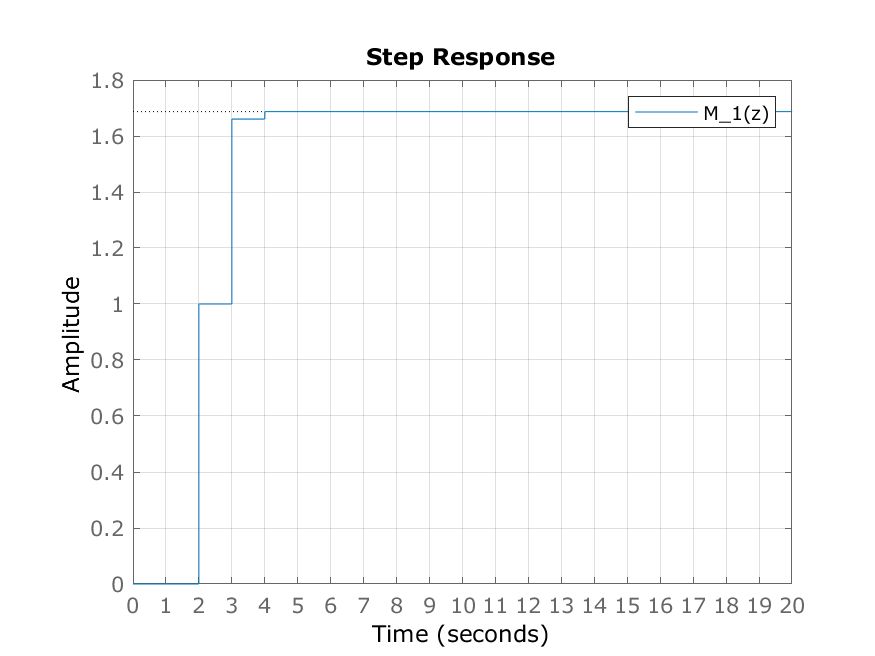
\includegraphics[width=0.6\linewidth]{img/exsim5-g1-deadbeat-sim.png}
    \caption{Resposta do Sistema para o controlador Deadbeat para sistema \ref{eq:ex5-g1}}
\end{figure}

\subsection{Part 2}

Temos que $n = \#polos - \#zeros + \#zeros = 3  - 2 + 2 = 1$

\begin{equation}\label{eq:ex5-g2}
    G_2(z) = \sympy{sG2}
\end{equation}

A partir do qual foi obtido a seguinte resposta em malha fechada para a rampa unitária:

\begin{figure}[H]
    \centering
    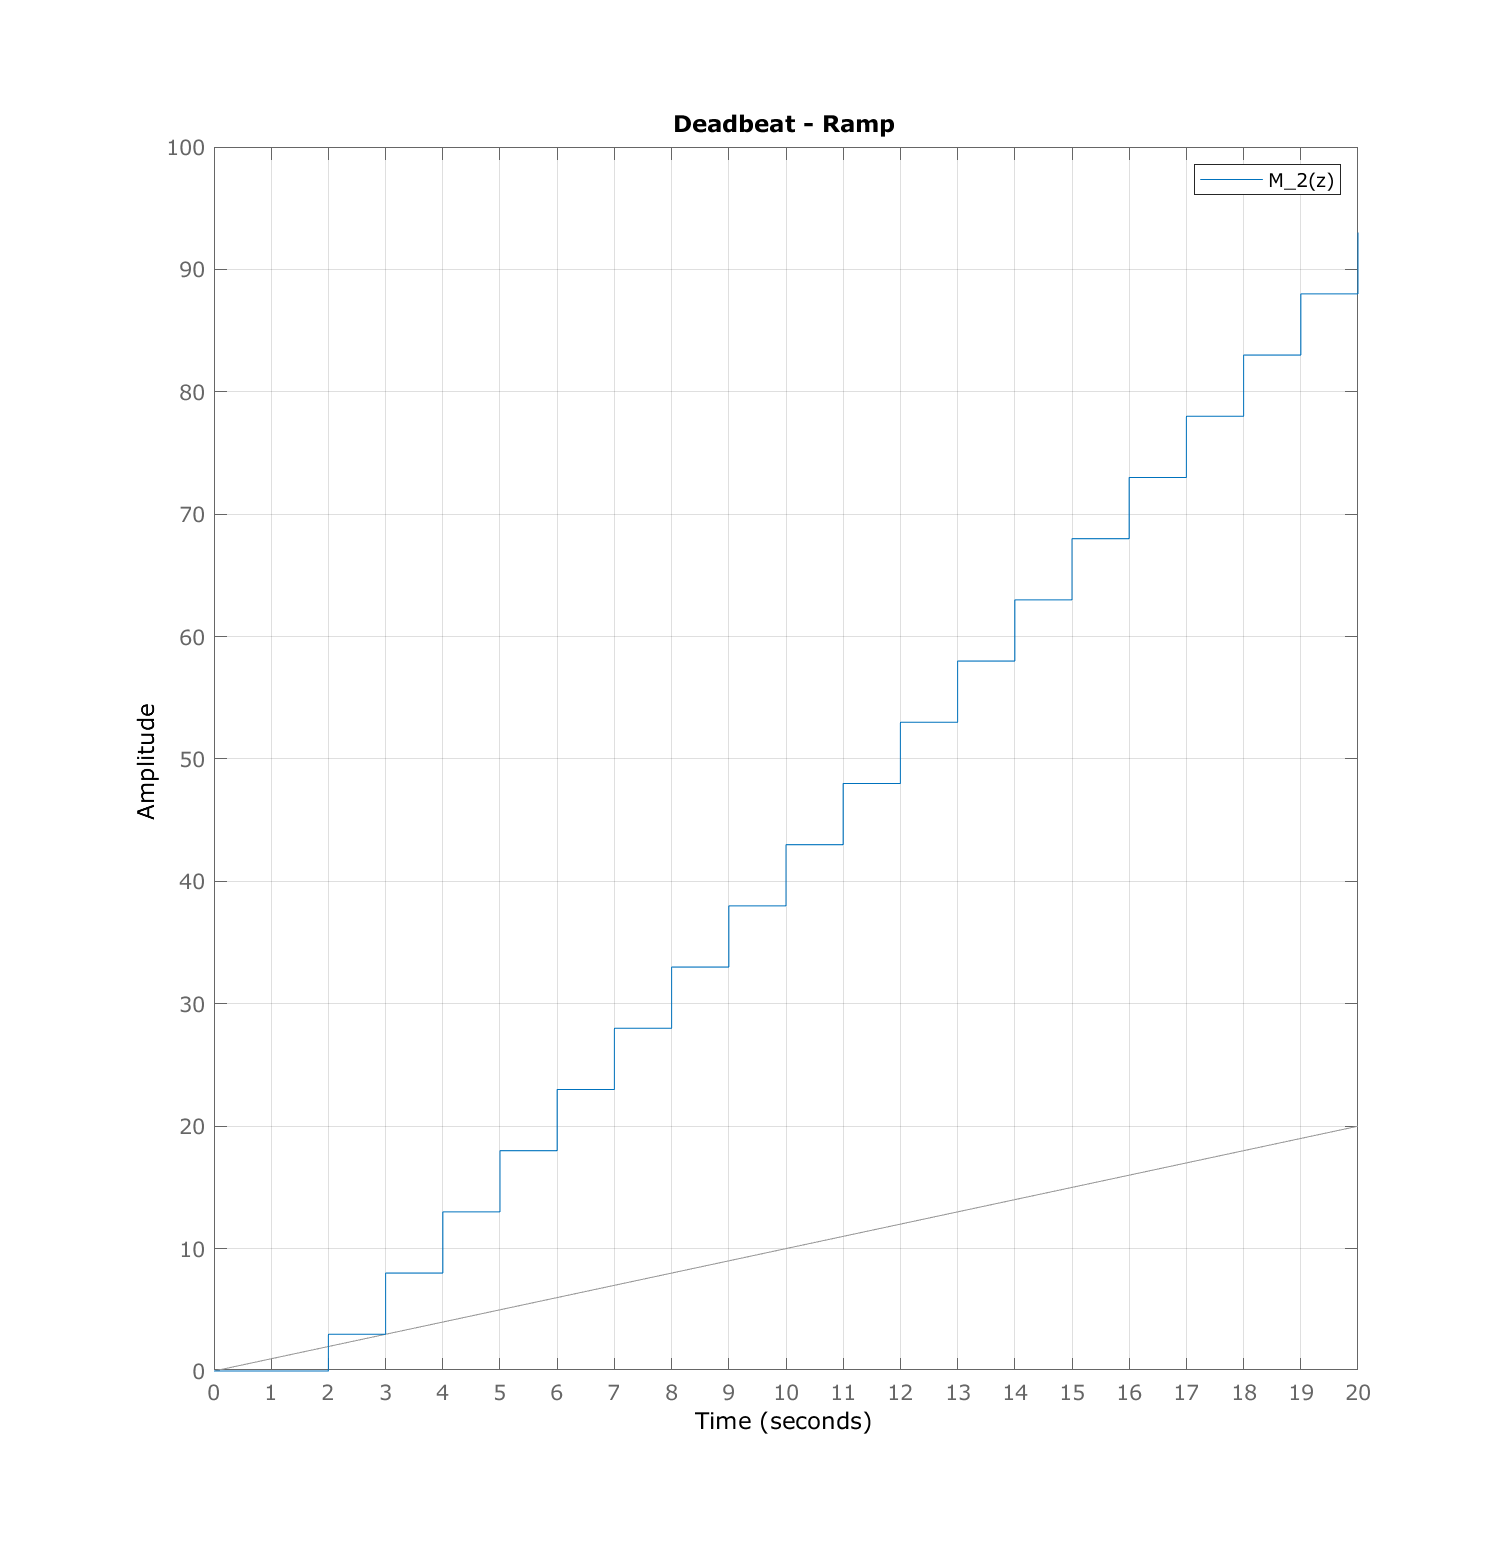
\includegraphics[width=0.6\linewidth]{img/exsim5-g2-deadbeat-sim.png}
    \caption{Resposta do Sistema para o controlador Deadbeat para sistema \ref{eq:ex5-g1}}
\end{figure}

\subsection{Part 1}

\begin{figure}[H]
    \centering
    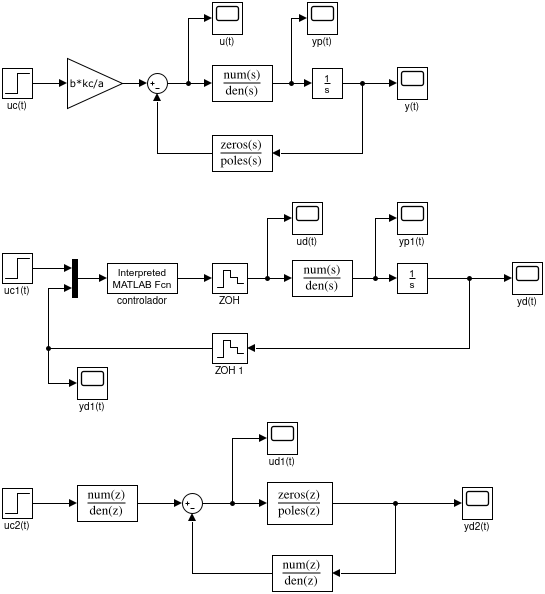
\includegraphics[width=0.9\linewidth]{img/exsim5model.png}
    \caption{Diagrama de Blocos do Sistema no Simulink - Planta exsim5}
\end{figure}


\subsubsection{}

Para o fins de comparação foi adotado a seguinte diagrama para o controle projetados para o exercício de simulação 2:

\begin{figure}[H]
    \centering
    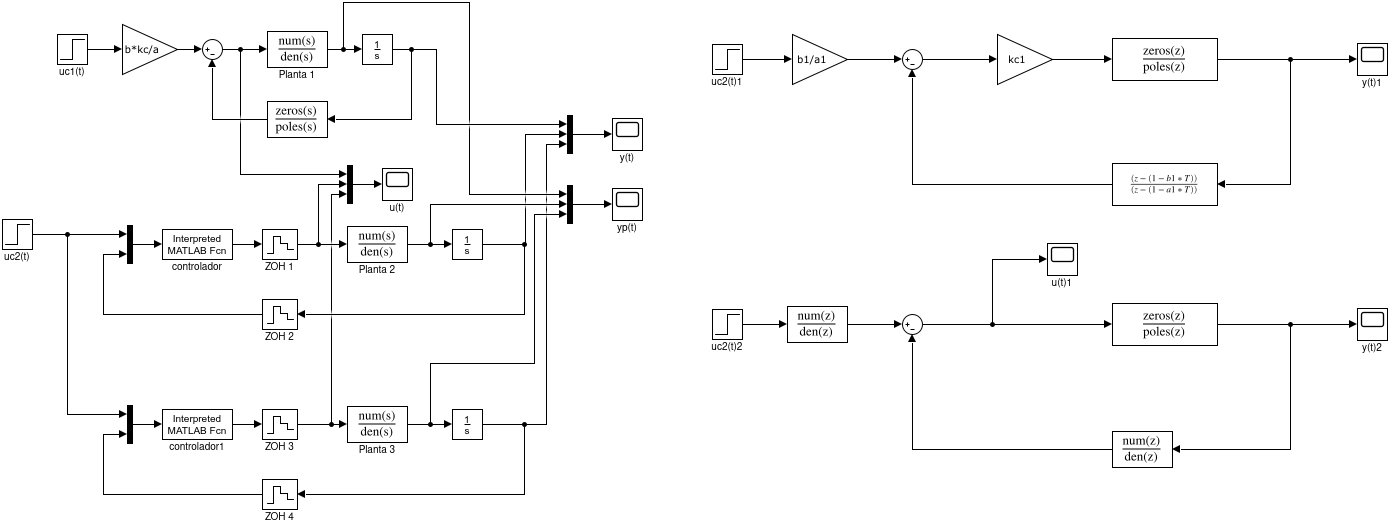
\includegraphics[width=1\linewidth]{img/exsim2model.png}
    \caption{Diagrama de Blocos do Sistema no Simulink - Planta exsim2}
\end{figure}

Com base nos valores definidos em script, foram obtidos os seguintes resultados para a simulação:

\begin{figure}[H]
    \centering
    \begin{subfigure}[m]{0.49\linewidth}
        \centering
        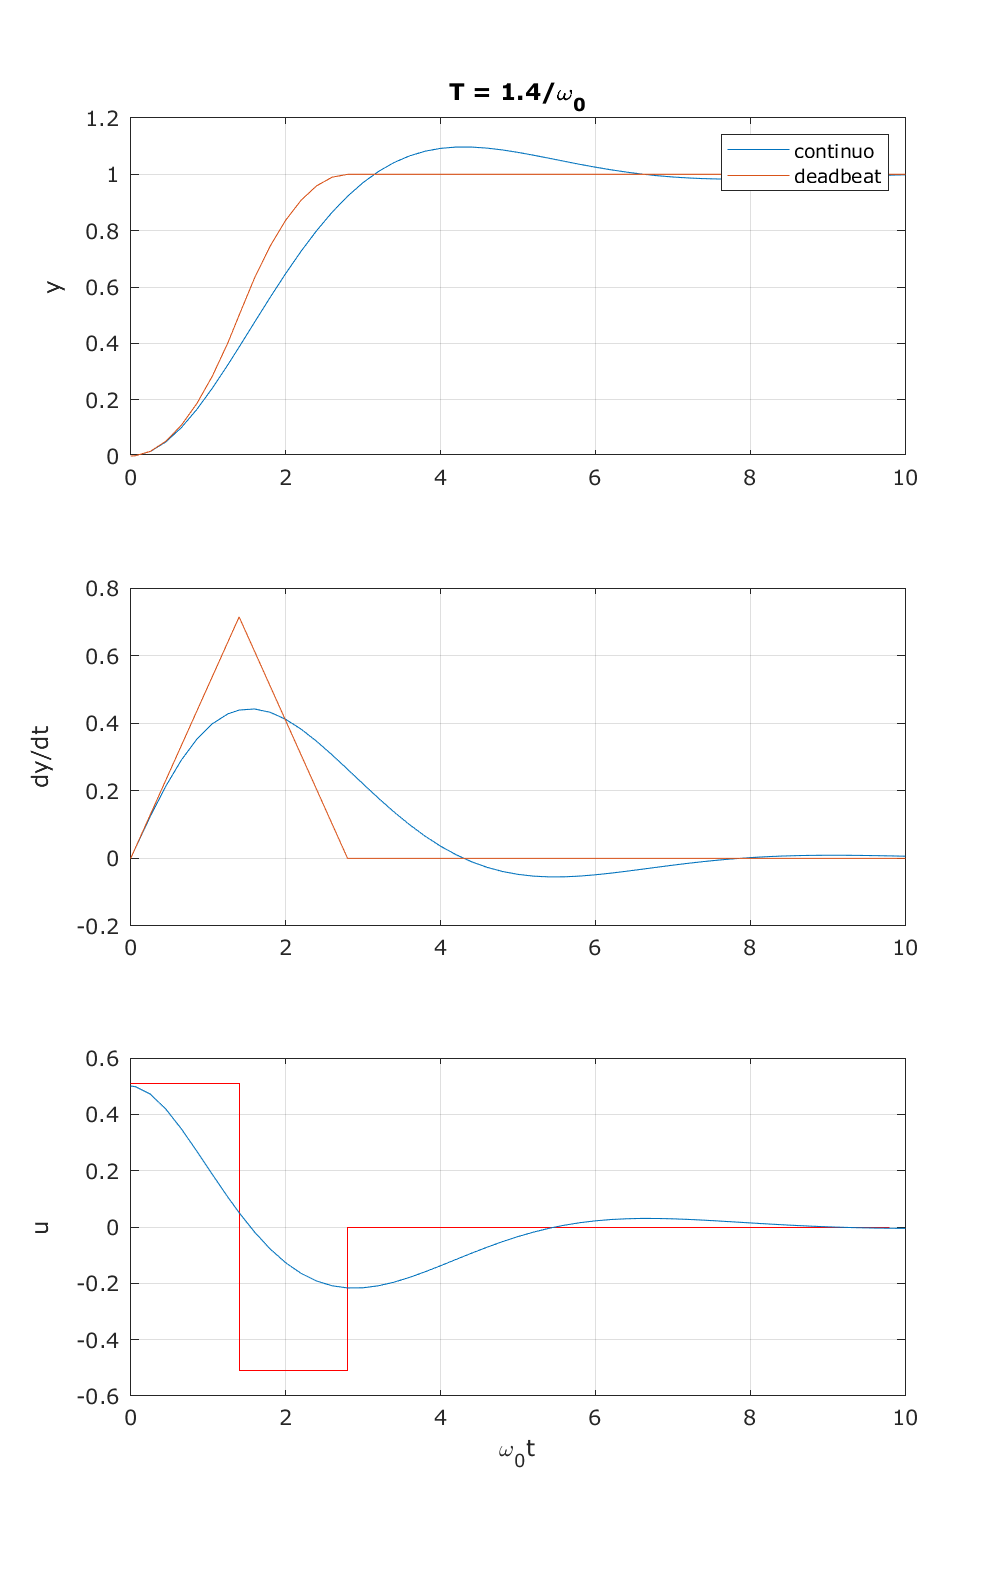
\includegraphics[width=1\linewidth]{img/exsim5-deadbeat-sim.png}
        \caption{Controlador Deadbeat - exsim5}
    \end{subfigure}
    \hfill
    \begin{subfigure}[m]{0.49\linewidth}
        \centering
        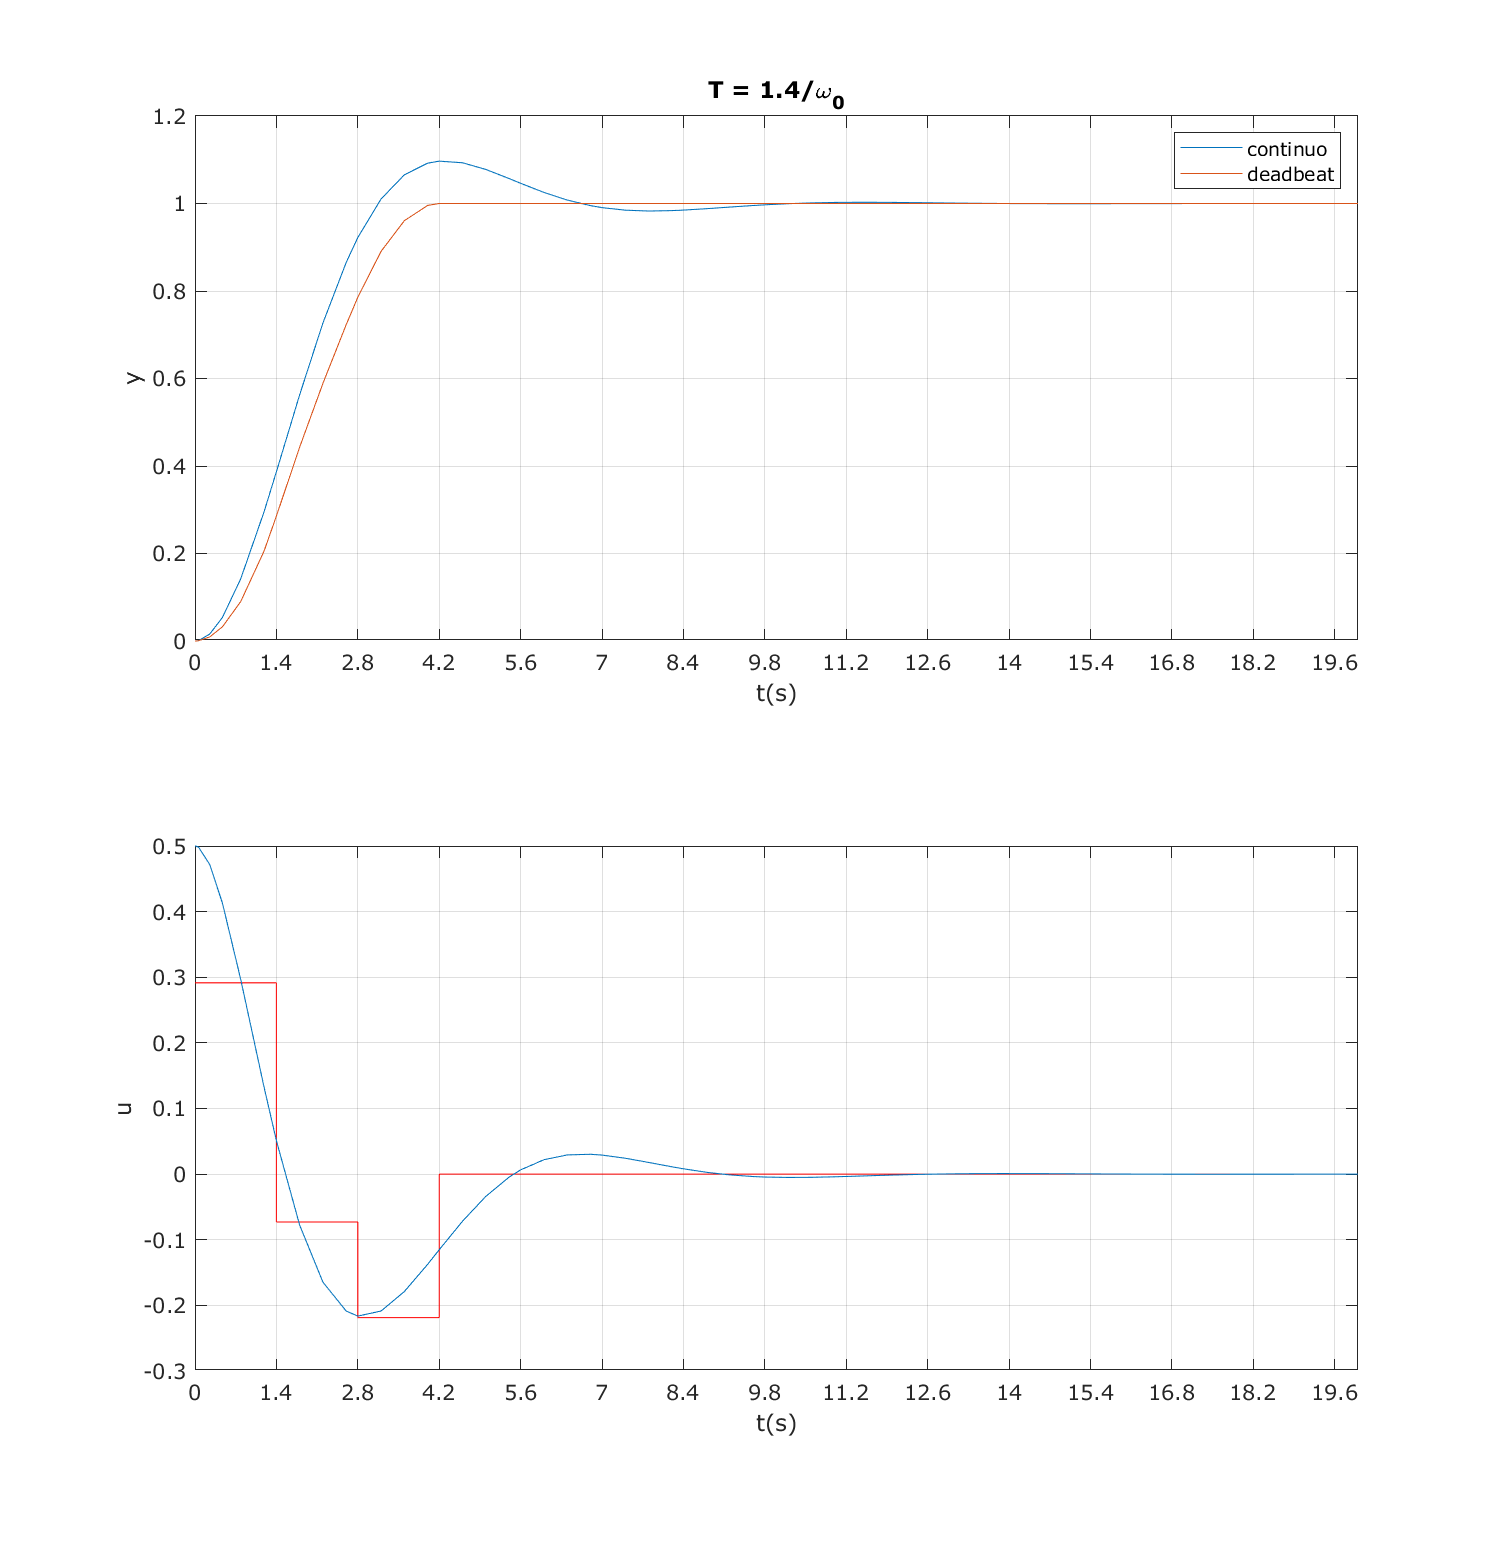
\includegraphics[width=1\linewidth]{img/exsim5-exsim2-sim.png}
        \caption{Controlador Discretizado - exsim2}
    \end{subfigure}
\end{figure}

Comparando ambas simulações percebemos que a metodologia adotada para o projeto do controlador na lanta exsim2 acaba levando mais tempo para estabilizar e têm um atraso em relação ao sistema contínuo. Enquanto para o controle da planta exsim5 é percebido uma resposta mais rápida e também uma ação de controle bme mais agressiva para um mesmo tempo de amostragem contando com uma varição bastante brusca do sinal passado para a planta. Algo que é característico de controladores deadbeat.

\section{Conclusão}


% ------------------------------------------------------------------------------
\newpage
% Referências
\addcontentsline{toc}{section}{Referências} % Adiciona linha no indice
\bibliographystyle{abbrv} % Define Estilo e gera bibliografia
\bibliography{references} % Adiciona Arquivo com Referências

% Acrescentadas no arquivo references.bib
% para usa-las no texto basta usar \citep{}
% para citar sem usar no texto basta usar \nocite{}
\nocite{sympy}
\nocite{pythontex}
\nocite{matlabcontrol}
\nocite{matlabsymbolic}
\nocite{ogata2010modern}

% ------------------------------------------------------------------------------
\newpage
\section*{Anexos}
\addcontentsline{toc}{section}{Anexos} % Adiciona linha no indice
\subsection*{Python}

Para os cálculos e demonstrações foi utilizado o pacote \textit{Python}\TeX\ \cite{pythontex} para o \LaTeX\ em conjunto da bibliteca \textit{sympy}\cite{sympy}. Segue o script completo em python:

\inputminted[xleftmargin=15pt,linenos,frame=single,framesep=5pt,breaklines=true]{python}{../python/exsim5.py}

\newpage
\subsection*{Matlab}

\subsubsection*{Parte 1}
Para o desenho dos gráficos e simulações foi utilizado o \textit{Matlab} em conjunto das toolbox \textit{Control System}\cite{matlabcontrol} e \textit{Symbolic Math}\cite{matlabsymbolic}. Segue o código referente usado

\inputminted[xleftmargin=15pt,linenos,frame=single,framesep=5pt,breaklines=true]{matlab}{../matlab/exsim5/exsim5.m}

\subsubsection*{Parte 3 - Controlador Dead Beat}
Para avaliação da resposta do controlador Dead Beat foi utilizado uma versão modificada dos script \textit{exsim5script} em \textit{Matlab} fornecido pelo professor:
\inputminted[xleftmargin=15pt,linenos,frame=single,framesep=5pt,breaklines=true]{matlab}{../matlab/exsim5/exsim5script.m}

\subsubsection*{Parte 3 - Controlador Discretizado}
Para comparativo com os resultados da simulação 2, foi utilizado uma versão modificada dos script \textit{exsim2script} em \textit{Matlab} fornecido pelo professor:
\inputminted[xleftmargin=15pt,linenos,frame=single,framesep=5pt,breaklines=true]{matlab}{../matlab/exsim5/exsim2script.m}



% ------------------------------------------------------------------------------
\end{document}
